% \section{Appendix}


\begin{table*}[htpb]
    \begin{tabular}{|l|l|l|l|l|l|}
    \hline
    Number of points & PSNR   & Mode     & Conv size & Pseudo color dimension & Multi-scale supervision \\ \hline
    100k             & 16.7dB & Bypass   & 1x1               & 3                      & Yes                     \\ \hline
    100k             & 21.2dB & Conv 5x5 & 5x5               & 3                      & Yes                     \\ \hline
    100k             & 26.3dB & Vanilla  & 5x5               & 8                      & No                      \\ \hline
    100k             & \textbf{29dB}   & Vanilla  & 5x5               & 8                      & Yes                     \\ \hline
    400k             & 23dB   & Bypass   & 1x1               & 3                      & No                      \\ \hline
    800k             & 25db   & Bypass   & 1x1               & 3                      & No                      \\ \hline
\end{tabular}
\caption{Quantitative performances (PSNR on validation set) of various training configurations on the \texttt{Old chair} scene.}
\label{tab:results}
\end{table*}


\begin{figure*}[htpb]
    \centering
    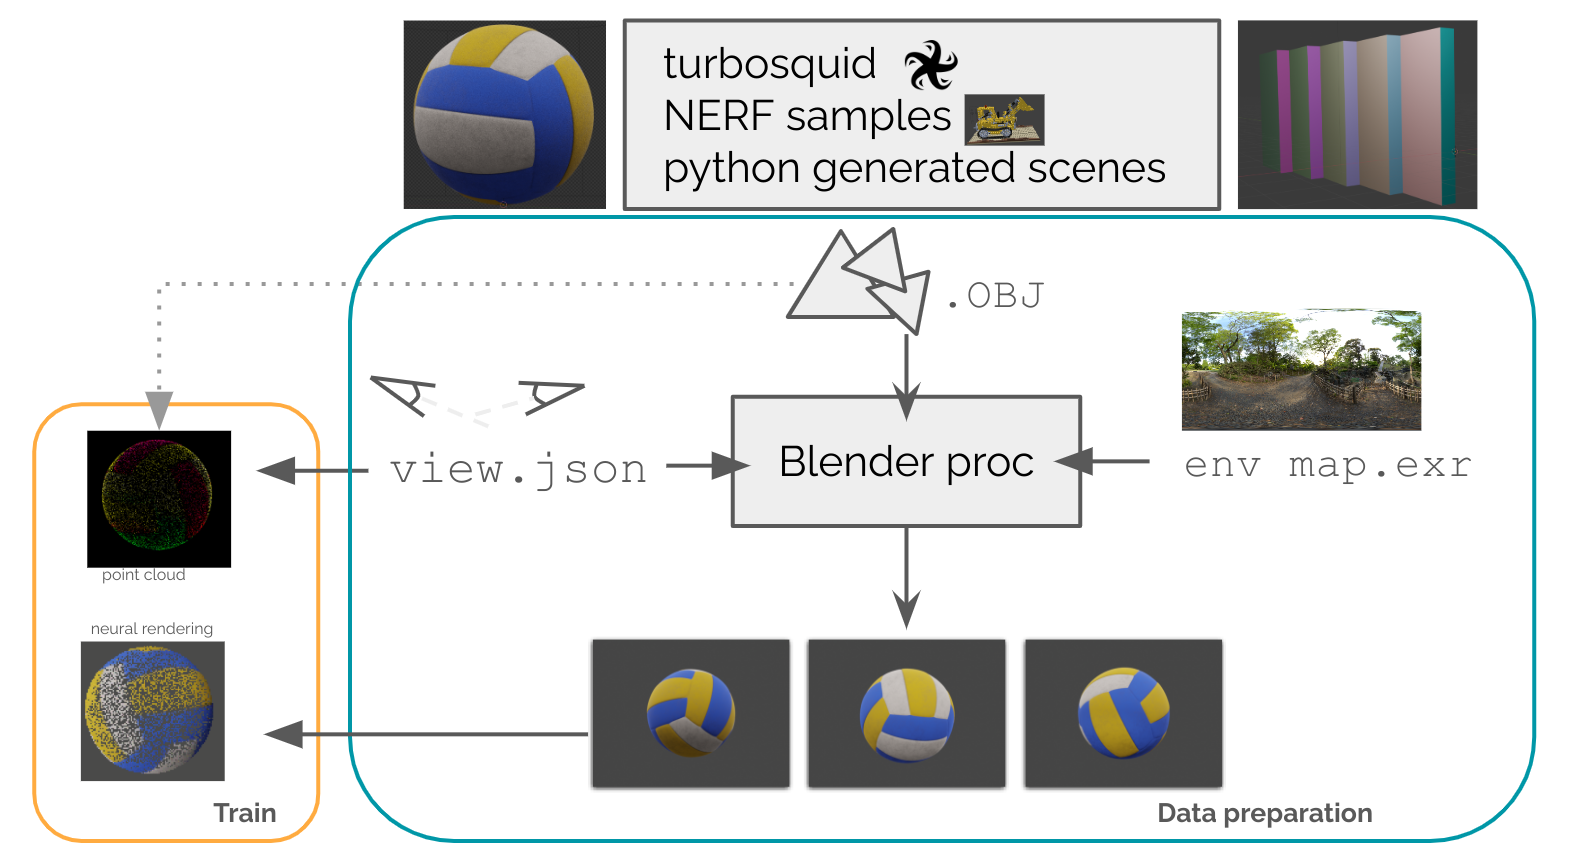
\includegraphics[width=0.5\textwidth]{figures/data_prep_and_training.png}
    \caption{Workflow: \href{https://github.com/balthazarneveu/per-pixel-point-rendering/blob/main/studies/photorealistic\_rendering.py}{\texttt{photorealistic\_rendering.py}} allows preparing camera multiviews positions saved as \texttt{.json} files in order to render photorealistic views of a \texttt{.blend} or  \texttt{.obj} files which come from internet resources or test scenes generated in python.
    The .obj and view .json files tie together the BlenderProc rendering and my Pytorch point rendering implementation: The point cloud is sampled from the mesh and the camera poses are known. A neural network is trained using \href{https://github.com/balthazarneveu/per-pixel-point-rendering/blob/main/scripts/optimize\_point\_based\_neural\_renderer.py}{\texttt{optimize\_point\_based\_neural\_renderer.py}} to predict colors of the points by trying to match the multiple photorealistic renderings. CNN weights, pointcloud, normals and pseudo-colors are all saved along in a \texttt{.pt} file which later allows performing live novel view synthesis \href{https://github.com/balthazarneveu/per-pixel-point-rendering/blob/main/scripts/novel\_views\_interactive.py}{\texttt{novel\_views\_interactive.py}} based on the self developped \href{https://github.com/balthazarneveu/interactive\_pipe}{interactive\_pipe} library}.
    \label{fig:data_and_train}
\end{figure*}

\begin{figure*}[htpb]
    \centering
    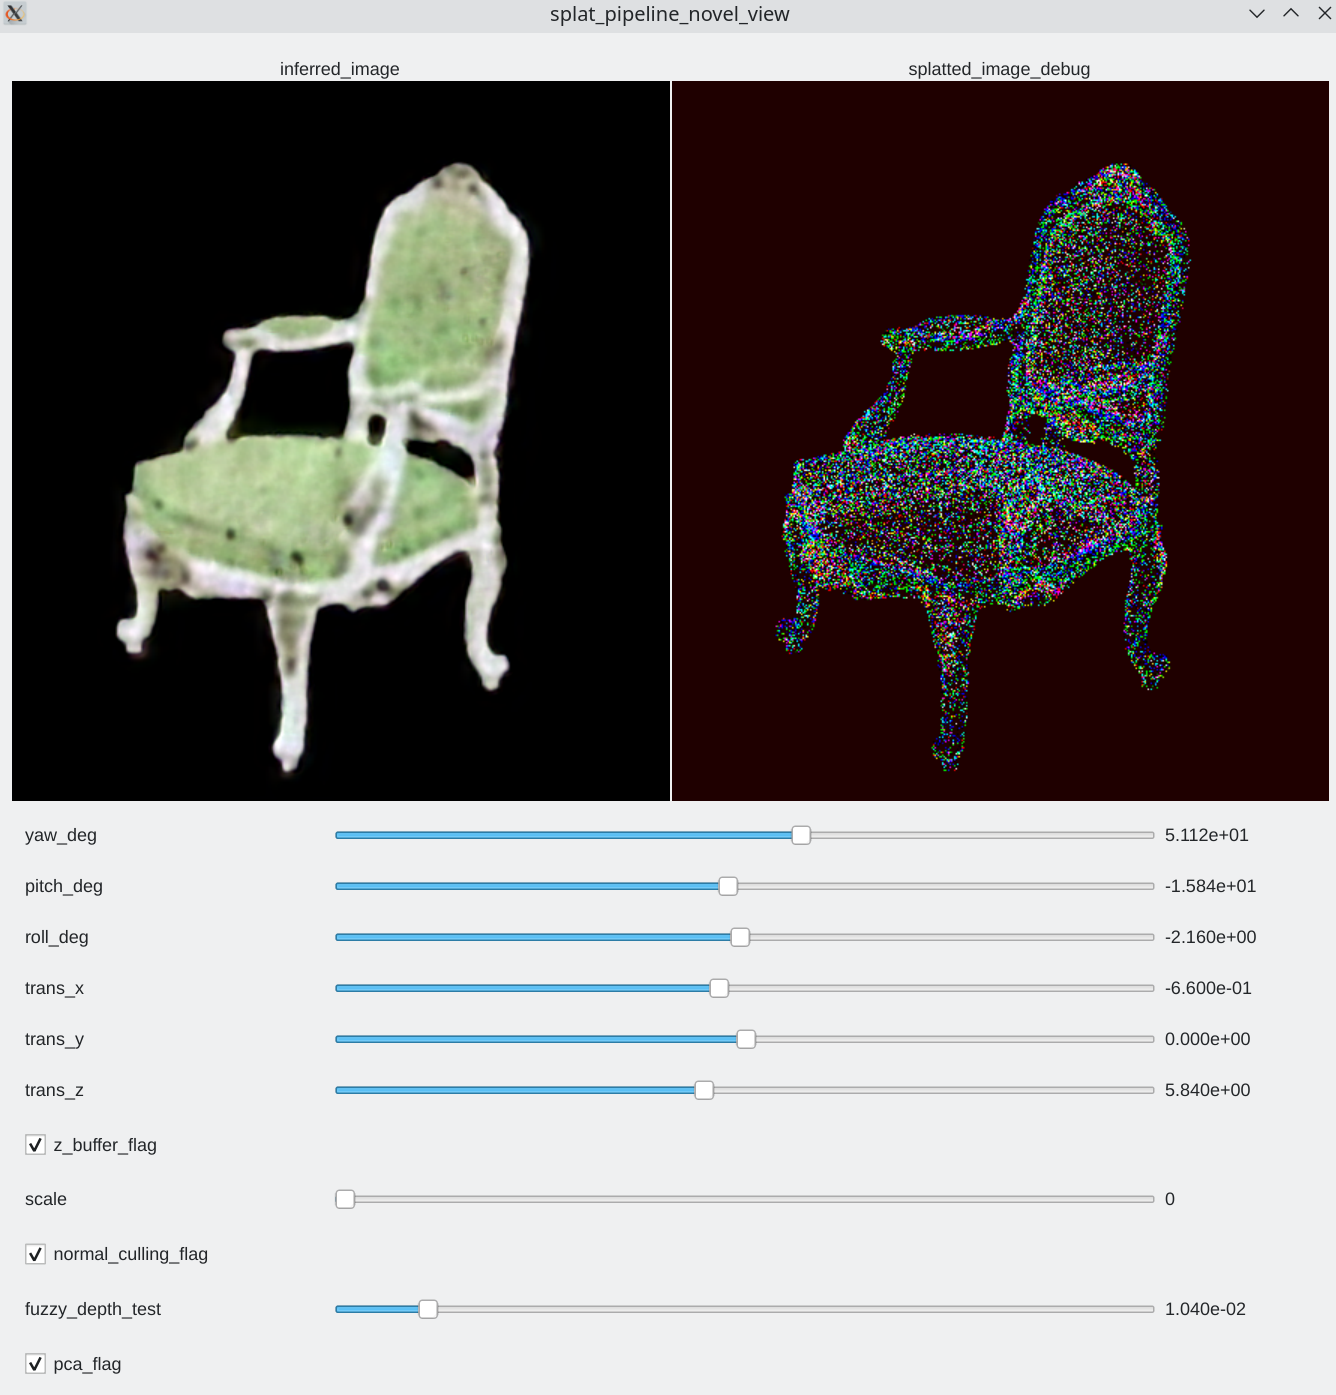
\includegraphics[width=0.4\textwidth]{figures/inference_live.png}
    \caption{Live inference, the user can move the camera around the scene and see the novel view rendered in real time. On the right side we visualize the projected pseudo colored point cloud of dimension 8 using a Principal Component Analyzis.}
    \label{fig:live_inference}
\end{figure*}


% \begin{table*}[htpb]
%     \begin{tabular}{|l|l|l|l|l|l|}
%     \hline
%     Number of points & PSNR   & Mode     & Conv size & Pseudo color dimension & Multi-scale supervision \\ \hline
%     100k             & 16.7dB & Bypass   & 1x1               & 3                      & Yes                     \\ \hline
%     100k             & 21.2dB & Conv 5x5 & 5x5               & 3                      & Yes                     \\ \hline
%     100k             & 26.3dB & Vanilla  & 5x5               & 8                      & No                      \\ \hline
%     100k             & \textbf{29dB}   & Vanilla  & 5x5               & 8                      & Yes                     \\ \hline
%     400k             & 23dB   & Bypass   & 1x1               & 3                      & No                      \\ \hline
%     800k             & 25db   & Bypass   & 1x1               & 3                      & No                      \\ \hline
% \end{tabular}
% \caption{Quantitative performances (PSNR on validation set) of various training configurations on the \texttt{Old chair} scene.}
% \label{tab:results}
% \end{table*}


% \begin{figure}[H]
%     \centering
%     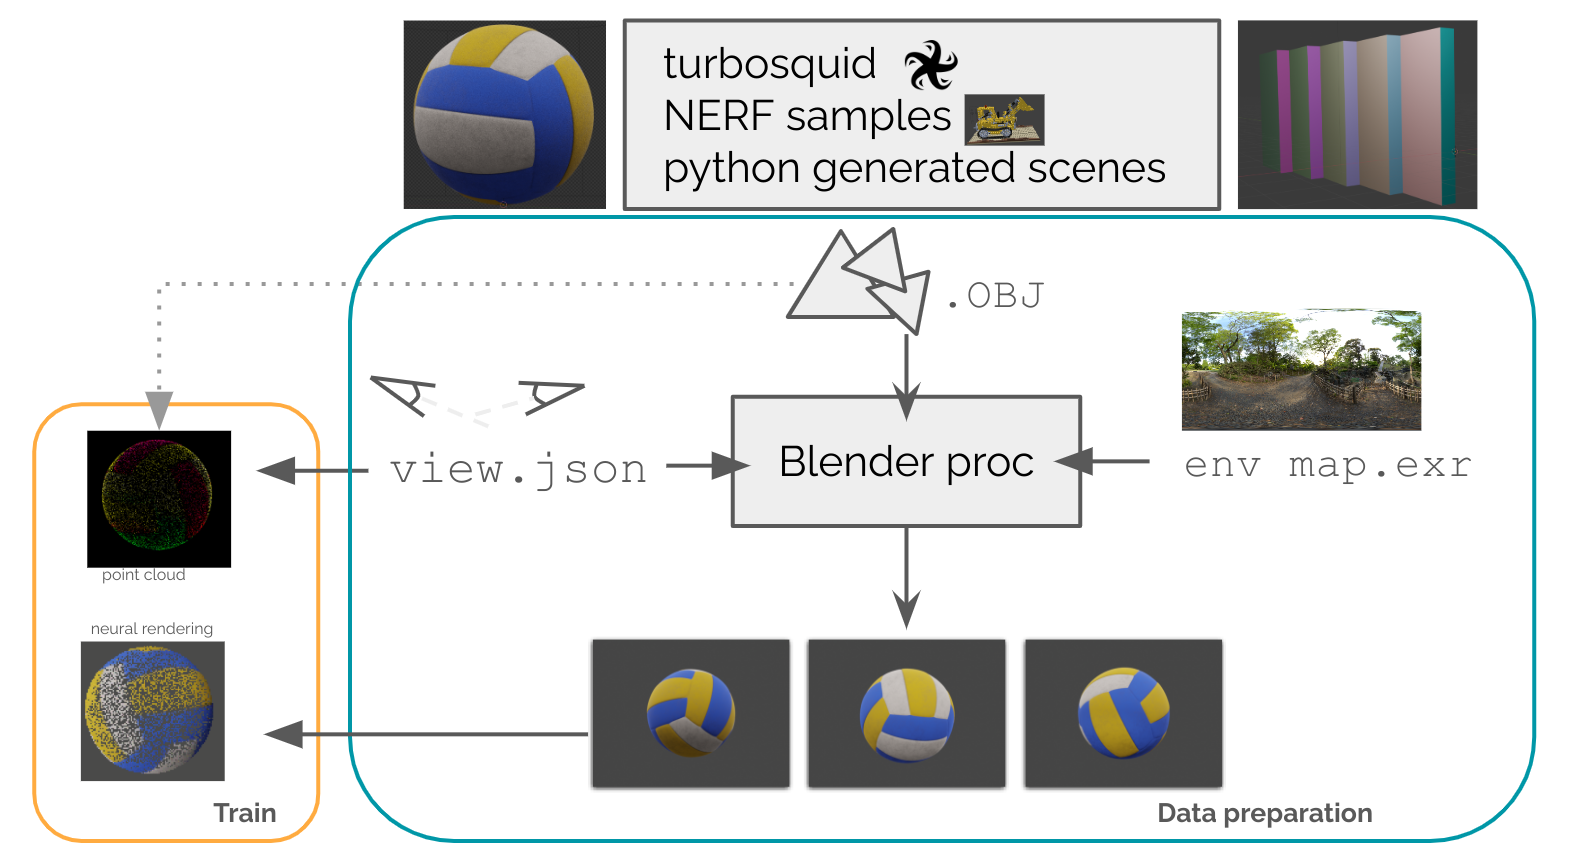
\includegraphics[width=0.45\textwidth]{figures/data_prep_and_training.png}
%     \caption{Workflow: \href{https://github.com/balthazarneveu/per-pixel-point-rendering/blob/main/studies/photorealistic\_rendering.py}{\texttt{photorealistic\_rendering.py}} allows preparing camera multiviews positions saved as \texttt{.json} files in order to render photorealistic views of a \texttt{.blend} or  \texttt{.obj} files which come from internet resources or test scenes generated in python.
%     The .obj and view .json files tie together the BlenderProc rendering and my Pytorch point rendering implementation: The point cloud is sampled from the mesh and the camera poses are known. A neural network is trained using \href{https://github.com/balthazarneveu/per-pixel-point-rendering/blob/main/scripts/optimize\_point\_based\_neural\_renderer.py}{\texttt{optimize\_point\_based\_neural\_renderer.py}} to predict colors of the points by trying to match the multiple photorealistic renderings. CNN weights, pointcloud, normals and pseudo-colors are all saved along in a \texttt{.pt} file which later allows performing live novel view synthesis \href{https://github.com/balthazarneveu/per-pixel-point-rendering/blob/main/scripts/novel\_views\_interactive.py}{\texttt{novel\_views\_interactive.py}} based on the self developped \href{https://github.com/balthazarneveu/interactive\_pipe}{interactive\_pipe} library}.
%     \label{fig:data_and_train}
% \end{figure}


% \begin{figure}[htpb]
%     \centering
%     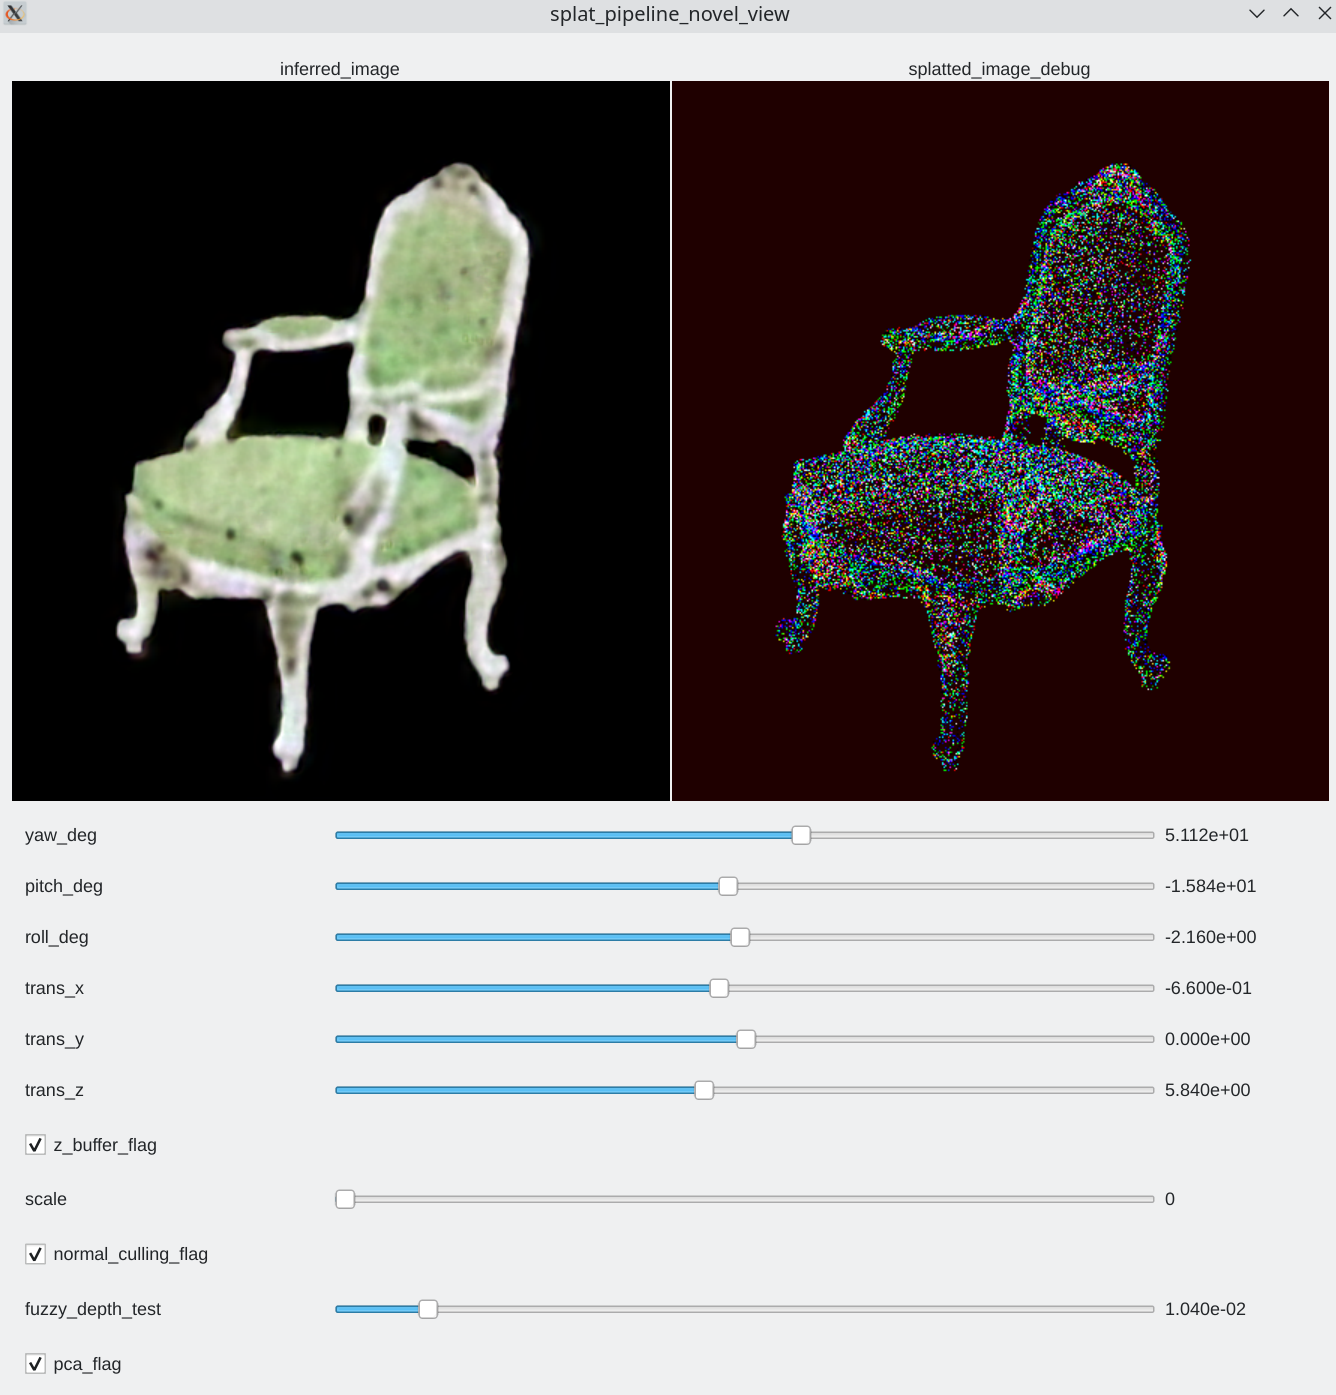
\includegraphics[width=0.45\textwidth]{figures/inference_live.png}
%     \caption{Live inference, the user can move the camera around the scene and see the novel view rendered in real time. On the right side we visualize the projected pseudo colored point cloud of dimension 8 using a Principal Component Analyzis.}
%     \label{fig:live_inference}
% \end{figure}
